\section{Rendering Pass}

实时且更复杂的渲染效果是在场景几何体上借助多次渲染来达到效果,这就是Rendering Pass的核心

\subsection{它是什么呢?}

它是一个模糊的概念,根具体的技术方案联系在一起。在OpenGL时代,一个rendering pass就是走完一遍渲染管线,从VS(Vertex Shader)到TS,
到GS, 到光栅化Rasterize,最后到FS中,得到的这一帧数据,是放在FBO或RT中,作为输入供
后面的pass使用。从一个rendering pass应该是一个RT来理解,与功能的需求相对应起来,是比较清晰的。

\par
RT与MRT,Tech

\par
在下一代图像API中,Vulkan把这些概念抽象为了具体的实体对象,使渲染的代码结构更加清晰,是因为当前
所有的GPU都在向tile-based,RenderPass的含义也是存在差异的,因为tile-based的原因,shader是隔离的
,所有的shader都是针对具体的像素范围,不能依赖邻居的shader值。\cite{gdc2020Arm}

\subsection{Refection Mapping}
反射映射是multipass最简单的例子,让一个被渲染对象被镜面化,并反射出场景中其他对象。
流程是首先渲染场景的其余部分,从渲染对象的中心观看的结果,即已中心为视点渲染6个图像,
\text{分别看向左、右、前、后、上、下六个图像},
\text{每个图像都是90度的垂直和水平视域(field of view)},
得到的数据就是一个cubeMap, 虽然这样的计算并非完全正确,但是给人一种可信的画面了,真正的反射是从
渲染对象的每一个点观察到合适的反射射线。

\subsection{Shadow Mapping}
阴影映射,在简单光照模型中,一个顶点上的色彩值不依赖场景中剩余的渲染对象,而真实世界中,
在表面点(顶点的法线的垂直面)与光源之间存在一个遮挡的对象,那么这个顶点就处于阴影中,会显得更暗些。

为实现这种情况下的真实性,借助multipass来模拟,思路是首先从光的视角生成并存储一个zBuffer的纹理,
随后从视角所看到与从光源视角看到的进行比较,如果从视角中看到的点而从光源视角没有看到,那么这个顶点
一定被某对象遮挡住。思路首先从光源视角渲染一个FBO,只存储深度值的FBO,再从视角渲染场景,对每个点与
存储在FBO中的深度值与当前顶点的深度值比较。


\subsubsection{Shadow Map}

可参考Advanced Lighting\cite{LearnOpenGL}

创建阴影的步骤:
\paragraph{一} 
以光源为视点,投影渲染整个场景,得到深度图ShadowMap并保存变换矩阵。ShadowMap中以光源为视点
时,所有可视点的深度。注意投影的区别:如果是DirectionLight则是正交投影,如果是PointLight,SpotLight则是透视投影

\paragraph{二}
以相机为视点渲染,对场景中的每个顶点,将其变换到以光源为视点的空间,若其深度大于ShadowMap中对应点
深度值,说明光源射来的光线被物体遮挡了,则该点处于阴影中。

运用渲染到纹理方法render to target,以场景中的光源为坐标原点,建立光源坐标系,就是场景深度
把render target(一般是R32F的surface)就是Shadow Map。 

接着正常render frame buffer, 启用depth buffer,将场景中的世界坐标的物体转化到以光源为基准的
投影坐标系中

世界坐标 $\rightarrow$ 物体坐标 $\rightarrow$ 光源坐标 $\rightarrow$ 光源视图坐标 $\rightarrow$ 光源投影坐标

任何在fragment shader中比较深度值,深度值小于shadow map对应的深度,就是光源照射地方,否则就是照射不到地方。
比较深度值时要把坐标转换为窗口坐标,因为shadow map是render to target的surface的结果。

\begin{itemize}
    \item [优点] \text{不用像volume那样去计算所有对象形状,只产生一直map}
    \item [缺点] \text{阴影有锯齿,比较深度值时就两种值,有阴影1和无阴影0,在阴影的边缘0和1交替出现而产生锯齿}
\end{itemize}

\paragraph{Shadow acne}
\begin{center}
    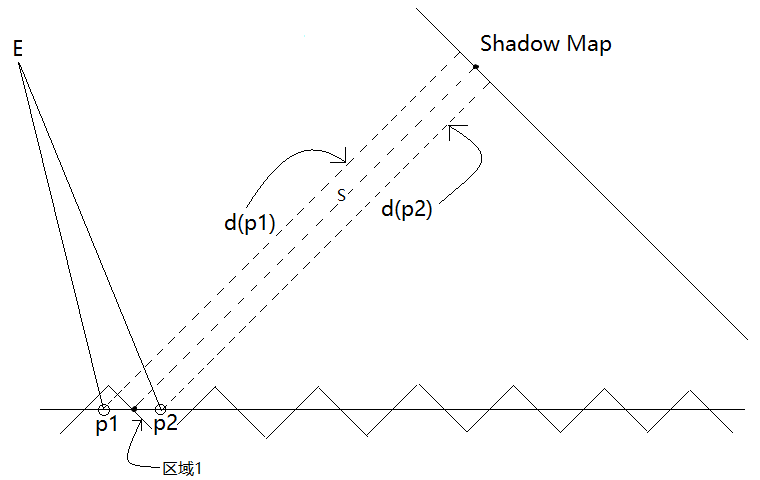
\includegraphics[width=0.4\textwidth]{images/shadow_acne.png}
    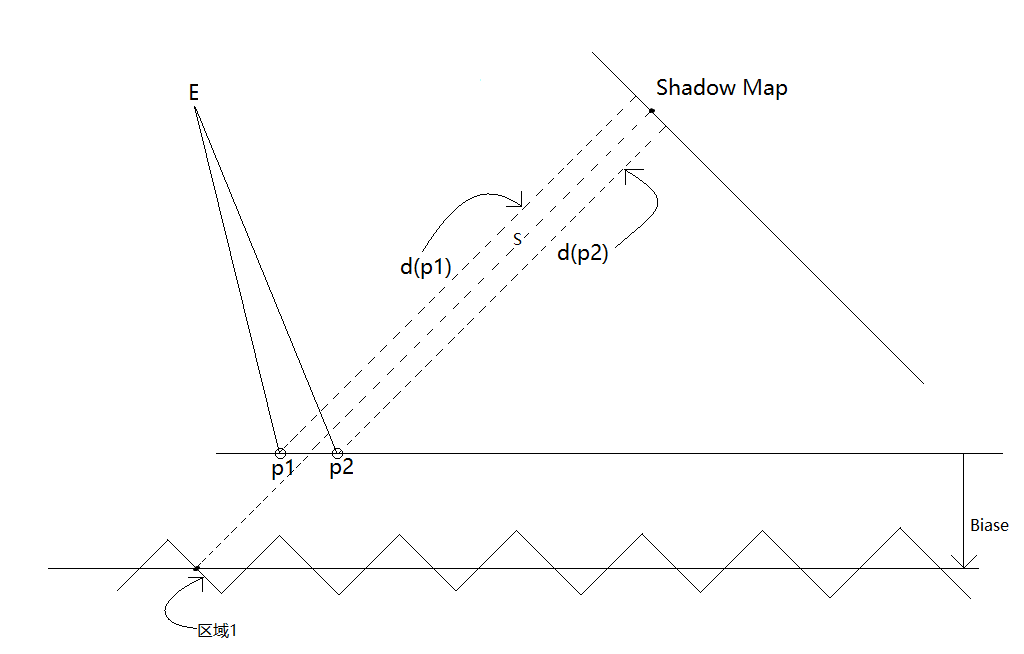
\includegraphics[width=0.4\textwidth]{images/shadow_acne_offset.png}
\end{center}
ShadowMap的分辨率有限,很容易产生阶梯状的边缘,每个Texel对应场景中的一个区域,如左边的图,点$p_{1}$和$p_{2}$对应屏幕上
不同的点,有$d(p_{1})>s, d(p_{2})<2$,点$p_{1}$也处在阴影中,解决的办法就是给shadow map中的深度值进行一个常量的偏移。

当三角形相对于光源而言,斜率过大,就需要一个非常大的偏移,就出现如下图所示的效果
\paragraph{Shadow Peter-pinning}
\begin{center}
    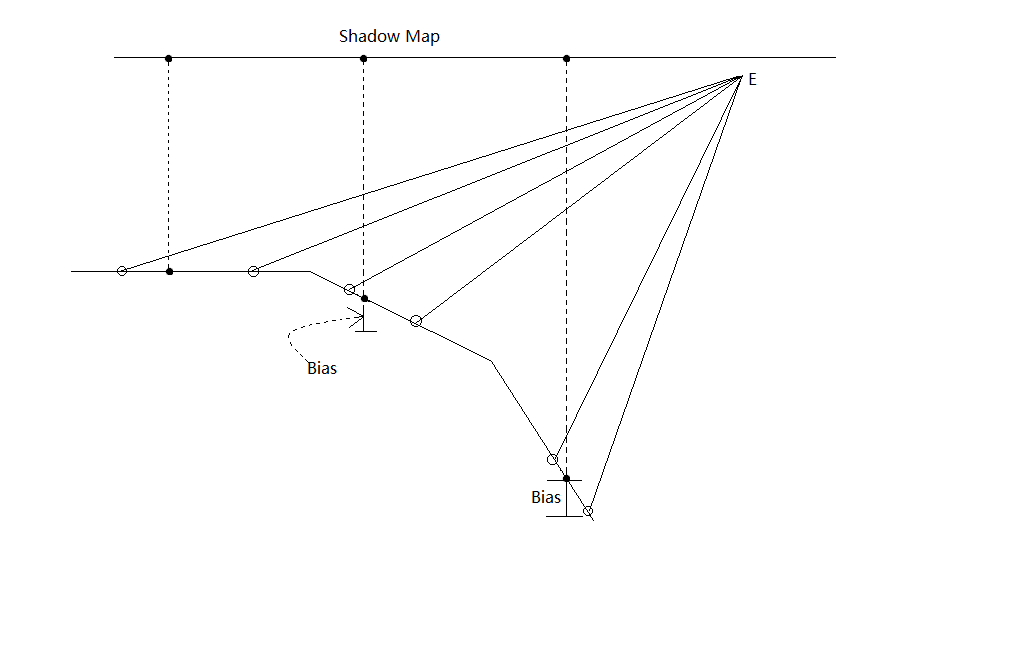
\includegraphics[width=0.8\textwidth]{images/shadow_peter-pinning.png}
\end{center}
为解决这种问题,图形显卡通过一种slope scaled bias的光栅化状态进行内置支持。

\paragraph{Shadow Bias}

\begin{gather*}
    bias = factorSlope \times slope + constantBias
\end{gather*}

\subsection{Hard \& Soft}

生成的阴影,其边缘没有过渡的,就会产生锯齿现象,而现实世界中的阴影边缘过渡得渐变很明显。
无渐变的shadow称为Hard Shadow,有渐变的称为Soft Shadow。为了产生渐变,就不能简单进行比较判断,得到是否的结果,
这就是shadow filtering的内容。

PCF(Perecentage Closer Filter), 将深度比较的结果0和1存储在一个render target里面,然后对其进行过滤操作,
产生值为0.2,0.5,...等灰度值的,即soft shadow。消耗时间较长,就简化成横向或纵向过滤,减少采样数量。

CSM(convolution shadow map), 此方法基于阴影重建,深度值比较的结果要么是1,要么是0,从而构造一个x坐标为[-1,1],
y坐标为[0,1]的函数,对函数进行FFT变换,运用基准函数sin和cos来重新构建shadow map。 

VSM(variance shadow map), 此方法应用切尔雪夫不等式,

\subsection{Perspective Aliasing}

近处锯齿现象,shadow map的分辨率不够。在camera视角下,近处的分辨率较高,一小片段对应着大量的pixel,而光源视角下的shadow map精度
并没有发生改变,就会大量的pixel对应着同一点,因而产生锯齿。 解决方案就是CSM(Cascaded Shadow Map),即一张不够,就多张来,
可参考微软的CSM\cite{CSM-msdn}
